\subsubsubsubsection{Traffic Light}
\begin{figure}[h]
\centering
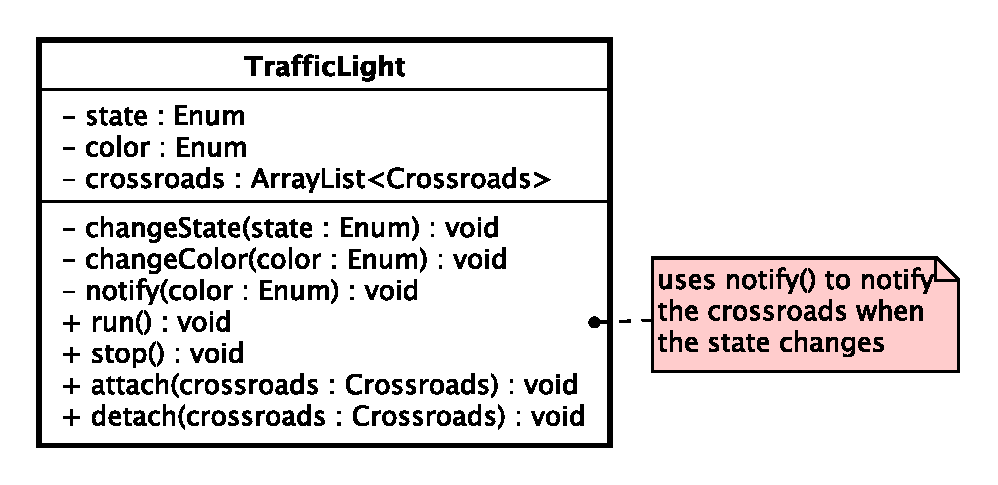
\includegraphics[scale=0.6,keepaspectratio]{images/solution/traffic_light.eps}
\caption{\pActive::TrafficLight}
\label{fig:sd-app-traffic-light}
\end{figure}
\FloatBarrier
\begin{itemize}
  \item \textbf{\descr} \\
    It represents an entity that has two possible colors (green, red) and switch
between them after a specified period of time. It is the subject of each 
crossroads/observer.
  \item \textbf{\attrs}
  \begin{itemize}
    \item \texttt{state: Enum} \\
The possible states of the entity \{ running, stopped \}.
    \item \texttt{color: Enum} \\
The possible colors of the entity \{ green, red \}.
    \item \texttt{crossroads: Collection<Crossroads>} \\
The observers that needs to be notified when the traffic light \textit{color} 
changes.
  \end{itemize}
  \item \textbf{\ops}
  \begin{itemize}
    \item[+] \texttt{TrafficLight(state : Enum, color : Enum)} \\
    Creates a traffic light specifying its state and color.
    \item \texttt{changeState(state: Enum)} \\
Change the entity state. This method is used internally by public methods to 
change the entity behaviour.
    \item \texttt{changeColor(color: Enum)} \\
Change the entity color. This method is used internally by public methods to 
switch between entity colors.
    \item \texttt{notify(color: Enum)} \\
Loops through the observer collection updating each crossroads state with the 
color passed as parameter. 
    \item[+] \texttt{run()} \\
Activates the entity which sets its state to \textit{running}. If its color is 
\textit{green} then it notifies the crossroads (passing the \textit{red} color)
and then changes its color to red, otherwise it changes its color to 
\textit{green} and then notifies the crossroad(passing the \textit{red} color).
After this process it waits for n seconds.    
    \item[+] \texttt{stop()} \\
Stops the entity which sets its state to \textit{stopped}.
    \item[+] \texttt{attach(crossroads: Crossroads)} \\
Adds the crossroads to the observer collection.
    \item[+] \texttt{detach(crossroads: Crossroads)} \\
Removes the crossroads from the observer collection.
  \end{itemize}
\end{itemize}
